\section{与经典积分的关系}
\label{sec:integ-classical}

新积分的定义与黎曼积分完全不同：一个切值域，一个切定义域。对熟悉的区间积分，两种定义给出的数是否相同，新积分又多处理了哪些函数？

本节分两种情形比较。有界闭区间上的有界函数，用不连续点集刻画黎曼可积性并证明两种积分相等；无界区间或奇点附近的反常积分，绝对收敛时与新积分一致，条件收敛时则不然。下文中区间上的测度都是Lebesgue测度$\lambda$。

\subsection{与黎曼积分的关系}
\label{sec:integ-riemann}

\paragraph{阶梯函数与上下和}
两种理论的接触点是阶梯函数。对区间$I\subseteq[a,b]$，$\int\mathbf 1_I\,\mathrm d\lambda=\lambda(I)$等于区间长度，与黎曼积分的值相同；端点是零测集，开闭不影响Lebesgue积分。由线性性，阶梯函数$\sum_ic_i\mathbf 1_{I_i}$的两种积分都等于$\sum_ic_i\lambda(I_i)$。而黎曼积分的上和与下和正是阶梯函数的积分，两种理论就从这里连起来。

回顾卷一的Darboux判据：有界函数$f$在$[a,b]$上黎曼可积，当且仅当对任意$\varepsilon>0$存在分割$P$，使上和与下和之差$U(f,P)-L(f,P)<\varepsilon$；此时黎曼积分是上下和共同逼近的值（可参考\BookChapterRef{chap:univariate-integration}{卷一第7章“一元函数的积分”}）。下面的判据把“上下和之差可以任意小”换成一个关于不连续点的测度条件。

\paragraph{振幅与不连续点}
上下和之差由函数在小段上的跳动幅度决定，所以要先量化函数在一点附近的跳动。设$f:[a,b]\to\mathbb R$有界，记$I_\delta(x)=(x-\delta,x+\delta)\cap[a,b]$，定义$f$在$x$处的\term{振幅}（oscillation）
\begin{equation}
 \omega_f(x)=\inf_{\delta>0}\Bigl(\sup_{I_\delta(x)}f-\inf_{I_\delta(x)}f\Bigr).
 \label{eq:integ-oscillation}
\end{equation}
括号内的量随$\delta$减小而不增，下确界就是$\delta\downarrow0$时的极限。$f$在$x$连续当且仅当$\omega_f(x)=0$，所以不连续点集为$D_f=\bigcup_{m\geq1}\{\omega_f\geq1/m\}$。例如$\mathbf 1_{[1/2,1]}$在$x=\frac12$处的振幅是$1$，在其余点都是$0$。

有了振幅，可以陈述下面的判据：决定黎曼可积性的是不连续点集的测度。

\begin{theorem}[黎曼可积的Lebesgue判据]
\label{thm:integ-riemann-lebesgue}
设$f:[a,b]\to\mathbb R$有界。$f$黎曼可积，当且仅当其不连续点集$D_f$是Lebesgue零测集。此时$f$关于Lebesgue可测集可测，Lebesgue可积，且$\int_{[a,b]}f\,\mathrm d\lambda$等于$f$的黎曼积分。
\end{theorem}

这一判据称为\term{Lebesgue判据}（Lebesgue criterion）。证明分三步：先说明黎曼可积函数被两列阶梯函数夹住，由此得到两种积分相等；再读出$D_f$零测；最后由$D_f$零测构造上下和之差很小的分割。下面始终记$\lvert f\rvert\leq M$。

\begin{proof}
\emph{第一步：两种积分相等。}设$f$黎曼可积。由Darboux判据，对每个$k$有分割$Q_k$使上下和之差小于$1/k$。令$P_k$为$Q_1,\dots,Q_k$的公共加细，加细不增大上下和之差，于是$P_1\subseteq P_2\subseteq\cdots$，且$U(f,P_k)-L(f,P_k)\to0$。

对$P_k$的每个小段$[x_{i-1},x_i]$，记$m_i,M_i$为$f$在其上的下、上确界，令$J_i=[x_{i-1},x_i)$（最后一段取闭区间），定义阶梯函数
\[
 \varphi_k=\sum_im_i\mathbf 1_{J_i},\qquad\psi_k=\sum_iM_i\mathbf 1_{J_i}.
\]
于是$\varphi_k\leq f\leq\psi_k$，并且
\[
 \int\varphi_k\,\mathrm d\lambda=L(f,P_k),\qquad\int\psi_k\,\mathrm d\lambda=U(f,P_k).
\]

分割加细时子段上的下确界不减、上确界不增，所以$\varphi_k$递增、$\psi_k$递减，分别有逐点极限$\varphi\leq f\leq\psi$，它们都是Borel可测函数。由$0\leq\psi-\varphi\leq\psi_k-\varphi_k$，得到
\[
 \int(\psi-\varphi)\,\mathrm d\lambda\leq U(f,P_k)-L(f,P_k)\to0 .
\]
所以$\psi=\varphi$在某个零测集$N$外成立，从而$f=\varphi$在$N$外成立。

集合$\{f>t\}$与Borel集$\{\varphi>t\}$只在$N$内可能不同，Lebesgue测度完备，所以$f$关于$\mathcal L$可测；又$\lvert f\rvert\leq M$，$f$在有限长区间上可积。$\varphi_k+M$是递增的非负简单函数，逐点收敛到$\varphi+M$，由引理~\ref{lem:integ-increasing-simple}，$\int(\varphi_k+M)\to\int(\varphi+M)$。两边减去有限数$M(b-a)$，得到
\[
 \int_{[a,b]}f\,\mathrm d\lambda=\int_{[a,b]}\varphi\,\mathrm d\lambda=\lim_kL(f,P_k)=\int_a^bf(x)\,\mathrm dx .
\]

\emph{第二步：$D_f$零测。}全部分割$P_k$的分点只有可数个，组成零测集$Z$。若$x\notin Z$，对每个$k$，$x$位于$P_k$某个小段的内部，存在$\delta$使$I_\delta(x)$含于该小段，于是
\[
 \omega_f(x)\leq M_i-m_i=\psi_k(x)-\varphi_k(x).
\]
令$k\to\infty$得$\omega_f(x)\leq\psi(x)-\varphi(x)$。在零测集$Z\cup N$之外右端为零，所以$D_f\subseteq Z\cup N$是零测集。

\emph{第三步：$D_f$零测蕴含黎曼可积。}给定$\varepsilon>0$，令$K=\{\omega_f\geq\varepsilon\}$。$K$是闭集：若$\omega_f(x)<\varepsilon$，取$\delta$使$I_\delta(x)$上上下确界之差小于$\varepsilon$，则对$\lvert y-x\rvert<\delta/2$有$I_{\delta/2}(y)\subseteq I_\delta(x)$，故$\omega_f(y)<\varepsilon$。

$K\subseteq D_f$是零测的有界闭集，可用可数个开区间覆盖且总长小于$\varepsilon$。$K$紧，取其中有限个，其并$G$由有限个不交开区间组成，总长小于$\varepsilon$。于是$[a,b]\setminus G$是有限个闭区间$H_1,\dots,H_r$之并，其上处处$\omega_f<\varepsilon$。

对每点$x\in H_l$取$\delta_x$，使$I_{\delta_x}(x)$上上下确界之差小于$\varepsilon$。区间$(x-\delta_x/2,x+\delta_x/2)$覆盖紧集$H_l$，取有限子覆盖，令$\delta$为相应$\delta_x/2$的最小值。若$H_l$中的小段$J$长度小于$\delta$，它含于某个$I_{\delta_x}(x)$，$f$在$J$上的上下确界之差小于$\varepsilon$。

把每个$H_l$分成长度小于$\delta$的小段，再加上$G$各分支的端点，得到分割$P$。上下和之差分两部分估计：落在某个$H_l$中的小段，每段的上下确界之差小于$\varepsilon$，总长不超过$b-a$，贡献小于$\varepsilon(b-a)$；落在$G$某个分支闭包中的小段，上下确界之差至多$2M$，总长小于$\varepsilon$，贡献至多$2M\varepsilon$。于是
\[
 U(f,P)-L(f,P)<\varepsilon(b-a+2M),
\]
由Darboux判据，$f$黎曼可积。
\end{proof}

第一步说明两种理论在共同范围内一致：黎曼可积函数的上下阶梯函数从两侧夹住它，Lebesgue积分记录了夹逼的公共极限。第二、三步说明黎曼可积的障碍恰好是不连续点占据正的长度。

这里用到了完备性。黎曼可积函数未必Borel可测，但与一个Borel函数只在零测集上不同，所以结论说的是关于Lebesgue可测集$\mathcal L$可测。

\paragraph{有理点指示函数}
在$[0,1]$上，有理点的指示函数$\mathbf 1_{\mathbb Q}$称为\term{Dirichlet函数}（Dirichlet function）。$\mathbb Q\cap[0,1]$可数，Lebesgue测度为零，所以
\[
 \int_{[0,1]}\mathbf 1_{\mathbb Q}\,\mathrm d\lambda=0 .
\]
另一方面，每个小区间上它的上确界为$1$、下确界为$0$，振幅处处为$1$，$D_f=[0,1]$的测度为$1$，所以它不黎曼可积。这与“任意分割的下和为$0$、上和为$1$”的直接计算一致。

图~\ref{fig:integ-dirichlet-function}把这个例子与Cantor集的指示函数放在一起。Cantor集$C$是零测的闭集，$\mathbf 1_C$在每个$x\notin C$的邻域内恒为零，因而连续；在$x\in C$处，由于$C$不含任何区间，$x$附近有取值为零的点，因而不连续。于是$D_f=C$不可数却零测，$\mathbf 1_C$黎曼可积，两种积分都是$0$。

\begin{BookInlineFigure}
  \centering
  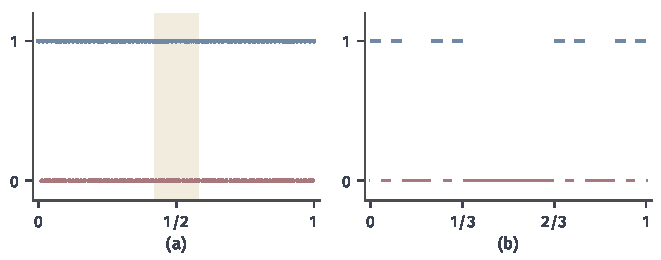
\includegraphics[width=112mm]{figures/04-spaces-measures-and-geometry/02-measure/matplotlib/integ-dirichlet-function/figure.pdf}
  \caption{两种不连续点集。(a)Dirichlet函数在有理点取$1$（蓝点）、无理点取$0$（红点），图中各取若干代表；两类点都稠密，任一小区间（黄色带）上上确界为$1$、下确界为$0$，不连续点集为整个$[0,1]$。(b)Cantor集的指示函数$\mathbf 1_C$，用第三步的$8$个保留区间示意$C$：蓝色线段处取$1$，红色线段处取$0$。它只在$C$上不连续，$\lambda(C)=0$，所以黎曼可积。}
  \label{fig:integ-dirichlet-function}
\end{BookInlineFigure}

两张图的对比说明，决定黎曼可积性的是不连续点集的测度，而不是它的基数或稠密性。$\mathbb Q$的基数比$C$小，$\mathbf 1_{\mathbb Q}$却不黎曼可积，因为它的不连续点集是全区间。Lebesgue积分则根本不要求函数在小区间上近似为常数，只要求各层可测。

\subsection{与反常积分的关系}
\label{sec:integ-improper}

\paragraph{截断区间的极限}
反常积分处理两种情形：区间无界，或函数在端点附近无界。做法都是先在有限闭区间上作黎曼积分，再让区间扩张取极限。新积分则直接在整个区间上累计，不需要截断。对非负函数，截断区间上的积分随区间扩张递增，这正是下一节单调收敛定理处理的情形。

\begin{theorem}[反常积分与Lebesgue积分]
\label{thm:integ-improper}
设$-\infty<a<\beta\leq+\infty$，$I=[a,\beta)$，$f:I\to\mathbb R$在每个$[a,b]$（$a<b<\beta$）上黎曼可积。
\begin{enumerate}
 \item 若$f\geq0$，则下式在$[0,+\infty]$中成立：
 \begin{equation}
  \int_If\,\mathrm d\lambda=\lim_{b\uparrow\beta}\int_a^bf(x)\,\mathrm dx .
  \label{eq:integ-improper}
 \end{equation}
 \item $f$在$I$上Lebesgue可积，当且仅当反常积分$\int_a^\beta\lvert f(x)\rvert\,\mathrm dx$收敛，即$\int_a^\beta f$绝对收敛；此时$\int_If\,\mathrm d\lambda$等于反常积分$\int_a^\beta f(x)\,\mathrm dx$。
\end{enumerate}
左端点为奇点的区间$(\alpha,b]$与两端都需截断的区间可类似处理。
\end{theorem}

证明的机制是：取$b_n\uparrow\beta$，截断函数$f\mathbf 1_{[a,b_n]}$逐点收敛到$f\mathbf 1_I$；当$f\geq0$时这列函数递增，积分与极限可以交换，而每个截断积分由定理~\ref{thm:integ-riemann-lebesgue}等于黎曼积分。交换的依据是单调收敛定理，所以完整证明放在第~\ref{sec:integ-monotone-convergence}小节，作为它的第一个应用。

对非负函数，反常积分收敛与Lebesgue可积是同一回事，值也相同。下面两个积分分别对应端点奇性和无界区间：
\[
\begin{aligned}
 \int_{(0,1]}x^{-1/2}\,\mathrm dx&=\lim_{\varepsilon\downarrow0}\bigl(2-2\sqrt\varepsilon\bigr)=2,\\
 \int_{[1,+\infty)}x^{-2}\,\mathrm dx&=\lim_{b\to+\infty}\Bigl(1-\frac1b\Bigr)=1 .
\end{aligned}
\]
对可正可负的函数，两种理论只在绝对收敛时一致；复值函数对实部和虚部分别使用第2条。

\paragraph{条件收敛不足以保证可积}
反常积分只要求截断积分有极限，允许正负部分相互抵消；Lebesgue积分则要求正负两部分各自有限。$f(x)=\sin x/x$在$[1,+\infty)$上体现了这一区别，图~\ref{fig:integ-sinc-improper}画出了它的前几瓣。

先看反常积分。分部积分得到
\[
 \int_1^b\frac{\sin x}x\,\mathrm dx=\cos1-\frac{\cos b}b-\int_1^b\frac{\cos x}{x^2}\,\mathrm dx .
\]
$b\to+\infty$时，$\cos b/b\to0$，而$\lvert\cos x/x^2\rvert\leq1/x^2$在$[1,+\infty)$上可积，最后一项也有有限极限。所以反常积分存在。

再看绝对值。在第$k$瓣$[k\pi,(k+1)\pi]$（$k\geq1$）上，$1/x\geq1/((k+1)\pi)$，而$\lvert\sin x\rvert$在每一瓣上的积分都是$2$，所以
\[
 \int_{[1,+\infty)}\frac{\lvert\sin x\rvert}x\,\mathrm dx\geq\sum_{k=1}^\infty\frac2{(k+1)\pi}=+\infty .
\]
由定理~\ref{thm:integ-improper}，$f$不Lebesgue可积。

进一步，$\int f^+$与$\int f^-$都是$+\infty$。它们是$\int_1^bf^\pm$的极限，而$\int_1^bf^+-\int_1^bf^-$有有限极限；若其中一个有限，另一个也有限，与$\int\lvert f\rvert=+\infty$矛盾。因此$f$在$[1,+\infty)$上的Lebesgue积分不存在。

\begin{BookInlineFigure}
  \centering
  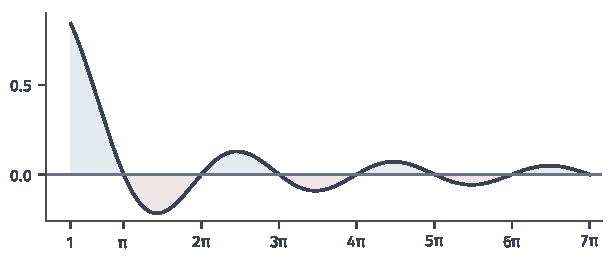
\includegraphics[width=104mm]{figures/04-spaces-measures-and-geometry/02-measure/matplotlib/integ-sinc-improper/figure.pdf}
  \caption{$f(x)=\sin x/x$在$[1,7\pi]$上的图像，正瓣蓝底、负瓣红底。第$k$瓣$[k\pi,(k+1)\pi]$上$\lvert f\rvert$的面积不小于$2/((k+1)\pi)$，各瓣面积之和按调和级数发散。按$x$增大的次序累加时正负瓣相互抵消，反常积分收敛。}
  \label{fig:integ-sinc-improper}
\end{BookInlineFigure}

图中正瓣与负瓣交替出现，面积按$1/k$缓慢减小。反常积分按从左到右的次序累加，正负瓣两两抵消，部分和收敛；把正瓣和负瓣分别累加，各自都发散。这与条件收敛的数项级数$\sum(-1)^k/k$相同：它的值依赖求和的次序。

测度积分不使用任何次序，所以它只接受与次序无关的绝对收敛情形。这并不是新积分的缺陷：需要条件收敛积分的场合，仍可以把它写成Lebesgue积分在截断区间上的极限。
